\chapter{Aero-elastic galloping}

\begin{center}
\colorbox{LightBlue}{\parbox{1\textwidth}{\noindent{\bf Note:} There is no need to repeat the information provided during the guided session. Answer the questions as concise and accurate as possible. Use graphical and/or tabular presentation rather than full sentences. The \textit{page limit} 
for this exercise is \textit{8 printed pages}, including figures.}}
\end{center}

A constant wind over a flexible, elastic structure can produce or sustain large amplitude oscillations,
as is testified by the Tacoma bridge disaster. One of the mechanisms that can cause this phenomenon is
aero-elastic galloping.\\

\begin{center}
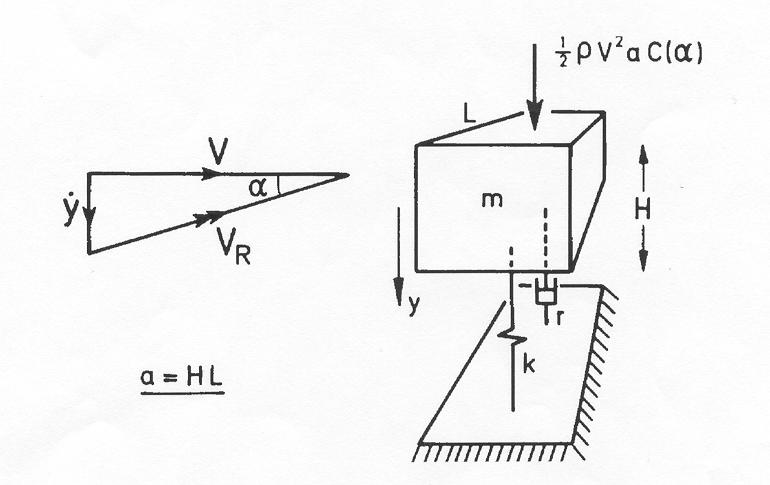
\includegraphics[scale=0.39]{gallop1.jpg}
%width=480pt,height=600pt
\end{center}

\noindent The square prism in the figure above represents an infinitesimal
element of a bridge. The forces that act on the element are:
\begin{itemize}

\item \textit{Inertia} : $m \ddot{y}$

\item \textit{Linear damping}: $r \dot{y}$

\item \textit{Elastic force}: $k y$

\item \textit{Driving force}: The wind speed $V_R$, relative to the prism, is composed of the prism's speed $\dot{y}$ and the constant absolute wind speed $V$. The resulting force depends of the angle $\alpha$ between the relative wind speed $V_R$ and the line perpendicular to the prisms direction of motion. For small $\alpha$, or equivalently large $V$, $\alpha$ can be approximated by $\alpha=\frac{\dot{y}}{V}$. The force along the \textit{direction of the speed} $\dot{y}$ is then given by
\[\frac{1}{2} {\rho V^2 a C(\alpha)}. \]
%(note the difference between $a$ and $\alpha$). We
\pj{We approximate} $C(\alpha)$ by the 7th order polynomial
\[C(\alpha)= A_1 \ \alpha - A_3 \ \alpha^3 + A_5 \ \alpha^5 - A_7 \ \alpha^7, \]
where $\alpha$ is expressed in radials and $A_1=0.04695$,
$A_3=8.932 \times 10^{-4}$, $A_5=1.015 \times 10^{-5}$ and $A_7=2.955 \times 10^{-8}$. Since the
driving force is a function of the speed $\dot{y}$, it can be seen
as a non-linear damping.
\end{itemize}

\noindent In the subsequent analysis, \pj{use} $m=1$, $\rho=1$, $r=1$, $k=100$ and $a=1$.

\begin{enumerate}

\item Write down the equations \pj{for the motion of the prism}. \rema{There is no need to discuss this in your report.}

\item Make a linear approximation of the model. Analyze the stability of \pj{possible} fixed
points as a function of the parameter $V$. At which critical wind speed $V_C$ do we have a bifurcation?
Identify the type of bifurcation of this linear model. Provide a tabular classification of the fixed point. \rema{Answer with a table.}

\item Make a model in \pj{\textsc{Matlab}} of the non-linear model (using the \verb!ode45! solver) where you gradually increase and decrease the parameter $\frac{V}{V_C}$ during the simulation.

\item When looking at the structure of $C(\alpha)$,
use your intuition to describe what will happen in the
neighbourhood of the bifurcation if the non-linear terms are not
neglected\pj{.} Verify using your \pj{\textsc{Matlab}}--model.

\item When $V$ grows larger than $V_C$ another bifurcation happens.
Lowering back $V$ shows the existence of a third bifurcation.
\pj{Identify the type(s) of these bifurcations.}

\textbf{Hint:} plot $y$ as a function of $\dot{y}$.

\item Use \verb!COCO! to obtain
\begin{enumerate}
	\item  a bifurcation diagram, plotting $\frac{A}{V_C}$ as a function of $\frac{V}{V_C}$, where $A$ is the maximal value of $y$ during a period, and
	\item  a plot of the periodic orbits in three dimensions (parameter $\frac{V}{V_C}$ and two phase space coordinates, e.g., $\frac{y}{V_C}$ and $\frac{\dot{y}}{V_C}$).
\end{enumerate}
\pj{Specify the parameters you used to compute the periodic orbits and perform the continuation.} \rema{Answer with some figures.}

\end{enumerate}

\noindent\pj{In the following, make sure that the orbit discretization is not changed between subsequent continuation steps (i.e., set \texttt{NAdapt} equal to \texttt{0}).}

\begin{enumerate}

\item[7.] \pj{The period of a limit cycle can be computed in \texttt{COCO} using}

\pj{\qquad\texttt{period = coco\_bd\_col(po\_data, \textquotesingle po.period\textquotesingle)}.}

\pj{Compute the period of the (first) limit cycle at $\frac{V}{V_C}=1.5$. Experiment with the number of subintervals \texttt{NTST} and the number of collocation points \texttt{NCOL} in each subinterval, while keeping all other parameters fixed. What is the effect on the computed period? Make a tabular representation of the relative error in the computed value for different combinations of \texttt{NTST} and \texttt{NCOL}, e.g., \texttt{NTST} $ \in \{6,12,24,48\}$ and \texttt{NCOL} $ \in \{3,5,7,9\}$. What do you observe?}  \rema{Answer with a table.}

\textbf{Hint:} set \texttt{TOL} to a sufficiently large value for the continuation, but do not change the value for the correction method.


%Implementation details: \\
%see \verb!MATCONT! short reference (by Frank Schilder)
%\begin{itemize}
%	\item  Initialising limit cycle continuation, 
%	\item  Computing branches of limit cycles,  
%	\item  Plotting Results (limit cycles): the function \verb plotcycle \ and computing solution measures. 
%\end{itemize}
%\item Show how the phase portrait evolves
%when varying $V$.  To this end, plot $\frac{\dot{y}}{V_C}$ with
%respect to $\frac{y}{V_C}$ for relevant values of $\frac{V}{V_C}$.

\end{enumerate}

\newpage

\newpage
